\documentclass[a4paper]{article}

\usepackage[sort]{natbib}
\usepackage{fancyhdr}


% \documentclass[a4paper]{article}

\usepackage[english]{babel}
\usepackage[utf8]{inputenc}
\usepackage{amsmath}
\usepackage{graphicx}
\usepackage[colorinlistoftodos]{todonotes}
\usepackage{hyperref}
\usepackage{booktabs} % To thicken table lines
\usepackage{tablefootnote}
\usepackage{listings}
% \usepackage[numbers]{natbib}

\usepackage{graphicx}
\usepackage{babel,blindtext}

\usepackage{algorithm}
\usepackage[noend]{algpseudocode}


% Uirá packages
\usepackage{algorithm}
\usepackage[noend]{algpseudocode}
\usepackage{booktabs} % To thicken table lines
\usepackage{graphicx}
\usepackage{babel,blindtext}
\usepackage{amsmath}
\usepackage[colorinlistoftodos]{todonotes}
\usepackage{hyperref}
\usepackage{mathtools}
\usepackage{listings}
\usepackage{epstopdf}



% you may include other packages here (next line)
\usepackage{enumitem}



%----- you must not change this -----------------
\oddsidemargin 0.2cm
\topmargin -1.0cm
\textheight 24.0cm
\textwidth 15.25cm
% \parindent=0pt
\parskip 1ex
\renewcommand{\baselinestretch}{1.1}
\pagestyle{fancy}
%----------------------------------------------------



% enter your details here----------------------------------

\lhead{\normalsize \textrm{Navigation}}
\chead{}
\rhead{\normalsize August 23, 2018}
\lfoot{\normalsize \textrm{DRLND - Udacity}}
\cfoot{}
\rfoot{Uirá Caiado}
\setlength{\fboxrule}{4pt}\setlength{\fboxsep}{2ex}
\renewcommand{\headrulewidth}{0.4pt}
\renewcommand{\footrulewidth}{0.4pt}


\begin{document}


%----------------your title below -----------------------------

\begin{center}

{\bf \large {Navigation Using Deep Reinforcement Learning \\ \small Uirá Caiado}}
\end{center}


%---------------- start of document body------------------

% The report clearly describes the learning algorithm, along with the chosen hyperparameters. It also describes the model architectures for any neural networks.

% A plot of rewards per episode is included to illustrate that the agent is able to receive an average reward (over 100 episodes) of at least +13. The submission reports the number of episodes needed to solve the environment.

According to \cite{spooner2016}, Reinforcement Learning (RL) is an area of machine learning that studies how a learner, called agent, interacts with an environment in order to maximize some notion of cumulative reward. As pointed out by \cite{mnih2015humanlevel}, to use RL successfully in complex environments, with high-dimensional state space, the agent must derive efficient representations of these inputs and use them to generalize past experience to new situations.

In this project, I trained an agent to navigate in a vast, square world, using Unity Machine Learning Agents Toolkit\footnote{Source: \url{https://github.com/Unity-Technologies/ml-agents}} to design, train, and evaluate Deep Reinforcement Learning algorithms. These algorithms combine RL with a class of artificial neural network, known as deep neural network, to generalize its past experiences to new ones. I considered to the tests the algorithms Deep Q-Learning (DQN) \cite{mnih2015humanlevel}, Double Deep Q-learning (DDQN) \cite{HasseltGS15} and DDQN with prioritized experience replay (PER) \cite{SchaulQAS15}.

The environment used for this project is the Udacity version of the Banana Collector environment, from Unity\footnote{Source: \url{https://youtu.be/heVMs3t9qSk}}. The goal of the agent is to collect as many yellow bananas as possible while avoiding blue bananas. The task is episodic, and to solve the environment, the agent must get an average score of +13 over 100 consecutive episodes.

A reward of +1 is provided for collecting a yellow banana, and a reward of -1 is provided for collecting a blue banana. The state space has 37 dimensions and contains the agent’s velocity, along with a ray-based perception of objects around agent’s forward direction. Given this information, the agent has to learn how to best select actions. Four discrete actions are available, corresponding to moving forward, backward, turn left and right.

% describes the model architectures for any neural networks
All the algorithms implemented in this project used the following architecture to the deep \textit{Q}-networks used. The input to the neural networks consists of an vector $37 \times 1$ produced by the environment. The input layer is a fully-connected linear layer with $128$ neurons and applies a rectifier nonlinearity. It is followed by a hidden layer also consisting of a fully-connected linear layer with $128$ neurons followed by another rectifier. The output layer is also a fully-connected linear layer with a single output for each action.

% (1) describes the learning algorithm, along with the chosen hyperparameters
% This algorithm was first introduced by \cite{mnih2015humanlevel} and combine RL with a class of artificial neural network known as deep neural network, using it to create a deep \textit{Q}-network $Q(s, a; \;\theta)$, with parameters $\theta$, to generalize its the past observations to new ones. The variables $s$ and $a$ stands for state and action.
The first algorithm tested was the vanilla DQN that was first introduced by \cite{mnih2015humanlevel}. As explained in the paper, the basic idea of many RL algorithm is to estimate the action-value function by using the Bellman equation as an iterative update, such that
\begin{gather*}
  Q^*(s, \, a) = \mathbf{E}_{s'} \left [r + \gamma \underset{a'}{\max} \, Q^{*} (s', a')|\,  s ,\, a\right ] \;,
\end{gather*}
where the variables $s$ and $a$ stands for state and action. In practice, it is common to use a function approximator to estimate the action-value function, $Q(s, a; \;\theta) \approx Q^*(s, \, a)$ ,  as a linear or a nonlinear function approximator, such as tile-coding and neural networks. In the paper, the neural network function approximator, called \textit{Q}-network, with weights $\theta$, is trained by adjusting its parameters to reduce the mean-squared error in the Bellman equation presented above. The Q-values $Q^{*} (s', a')$ in the equation are substituted with approximate Q-values $Q(s', a'; \;\theta^{-})$, using parameters $\theta^{-}$ from some previous iteration.

The paper modified the standard online \textit{Q}-learning in two ways to make it suitable for training large neural networks without diverging. First they used a experience replay buffer to store the agent's experiences at each time-step, $e_t = (s_t, a_t, r_t, s_{t+1})$, in a dataset $D_t = \{e_1, \cdots ,e_t\}$. These experiences are drawn at random from the buffer to apply the \textit{Q}-learning updates. Among the advantages cited in the paper, the authors suggested that learning from consecutive samples is inefficient, owing to the strong correlations between the samples, and randomizing the samples breaks the correlations and reduce the variance of the updates. The second modification introduced was to use a separate network with parameters $\theta^{-}$ for generating the targets in the Q-learning update, or mini-batch updates, and cloning every $C$ updates the parameters of the network $Q(s, a; \;\theta)$ to obtain the target network $Q(s, a; \;\theta^{-})$.

In this project, I introduced more two modifications. Fist, as suggested by Udacity, instead of cloning the current network to the target network, I used a "soft-update" to make the target network slightly closer to the $Q(s, a; \;\theta)$ using $\theta^{-}= \tau \theta + (1- \tau)\theta^{-} $. It guarantees that the target network is always different enough from the current "local" network. I used $\tau=0.001$. The other modification I introduced that was particularly helpful was clipping the reward to be between $-1$ and $1$.

I also used a buffer size of $100,000$ experiences, a mini-batch size of $64$, $\gamma=0.99$, the learning rate of $0.0005$ and updated the \textit{Q}-networks every four steps. Both local and target \textit{Q}-networks presented the same architecture, described before. Using this configuration, I was able to solve the environment in $529$ episodes. The figure \ref{fig:dqn} presents the results of the simulation. The left panel exposes the rewards obtained in each episode and, in the right panel, I plotted a moving average of the last $100$ episodes of this rewards. The shaded area corresponds to one standard deviation $\sigma$ of the rewards of those $100$ episodes.

\begin{figure}[ht]
\centering
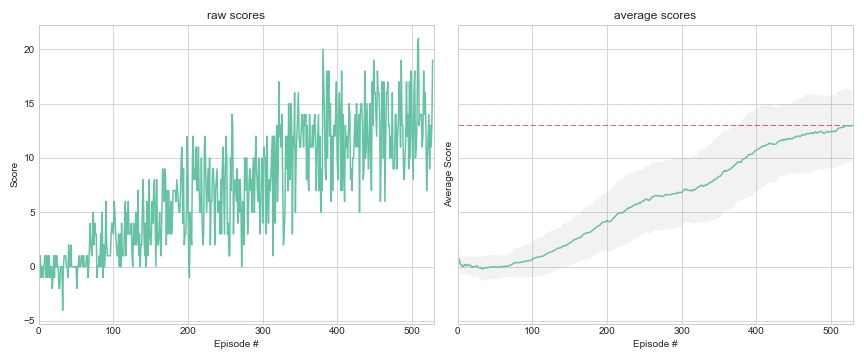
\includegraphics[width=0.65\textwidth]{../notebooks/figures/2018-08-24-dqn.jpg}
\caption{Learning Curve(left panel) and Moving-average(right panel)}
\label{fig:dqn}
\end{figure}


% (2) describes the learning algorithm, along with the chosen hyperparameters
The second model implemented and tested was the Double DQN (DDQN), that was first introduced by \cite{HasseltGS15}. As explained by the authors, the max operator in DQN uses the same values both to select and to evaluate an action, what makes it more likely to select overestimated values. Thus, the paper decomposes the action selection and the action evaluation by using the target network to evaluate the action chosen by the local network, such that
\begin{gather*}
  Y_t = r + \gamma Q (s', \underset{a'}{\arg \max} \, Q (s', a'; \theta);\theta^{-}) \;,
\end{gather*}
where $Y_t$ corresponds to the target value. Both networks must agree over the best action to the \textit{Q}-value returned to be the maximum one.

\begin{figure}[ht]
\centering
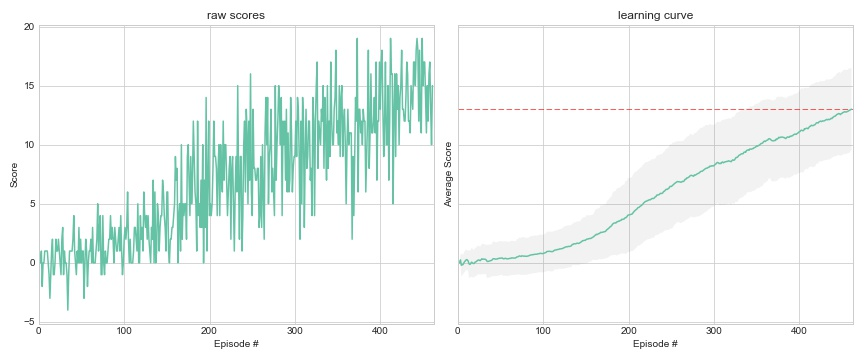
\includegraphics[width=0.60\textwidth]{../notebooks/figures/2018-08-24-ddqn-learning-curve.jpg}
\caption{Learning Curve(left panel) and Moving-average(right panel)}
\label{fig:ddqn}
\end{figure}

I used the same configurations of the tests with DQN and the model implemented was able to solve the task in $462$ episodes. The figure figure \ref{fig:ddqn} above presents the results.

% (3) describes the learning algorithm, along with the chosen hyperparameters
The last model tested was the prioritized experience replay presented by \cite{SchaulQAS15} and built on top of DDQN. Their key idea, well summarized by \cite{Wang:2015wz}, was to increase the replay probability of experience tuples that have a high expected learning progress, measure by the absolute TD-error of the step that collected that experience. 

The figure \ref{fig:ddqnper} presents the performance of the DDQN with PER. I used the same hiper-parameters of the previous model and includes the PER parameters importance sampling exponent $\alpha=0.6$ and prioritization exponent $\beta=0.4$. The values were chosen based on the original paper. The algorithms were able to solve the environment in $562$ episodes.


% A plot of rewards per episode is included to illustrate that the agent is able to receive an average reward (over 100 episodes) of at least +13
\begin{figure}[ht]
\centering
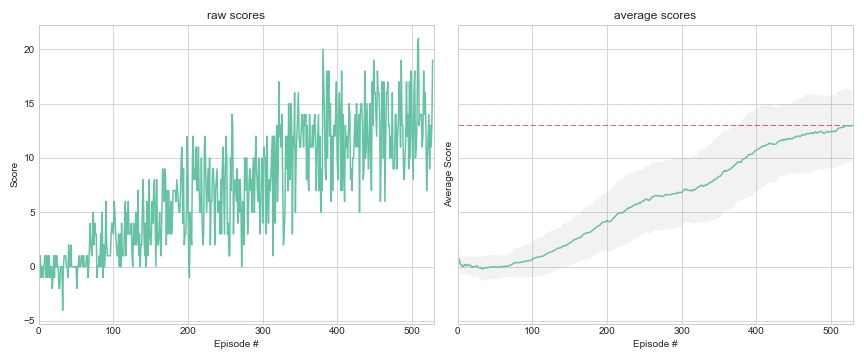
\includegraphics[width=0.65\textwidth]{../notebooks/figures/2018-08-23-ddqnpre-learning-curve.jpg}
\caption{Moving Average of $100$ episodes of the score}
\label{fig:ddqnper}
\end{figure}

 % The submission reports the number of episodes needed to solve the environment.


The table \ref{tab:final_results} below presents the final performance of each algorithm tested. The error margins were computed using the standard deviation of the distribution of the final score over the last $100$ episodes. The figure \ref{fig:final_comp} presents a comparison of the moving average of $100$ episodes of the scores achieved by each model.

\begin{table}[ht!]
\centering
\begin{tabular}{lrrr}
{model} &  episodes &  Score \\
\midrule
DDQN with PER &       562 &       $13.06\pm3.47$ \\
DDQN          &       462 &       $13.01\pm3.48$ \\
DQN           &       529 &       $13.01\pm3.42$ \\

\end{tabular}
\caption{\label{tab:final_results}Summary of the tests}
\end{table}
\begin{figure}[ht]
\centering
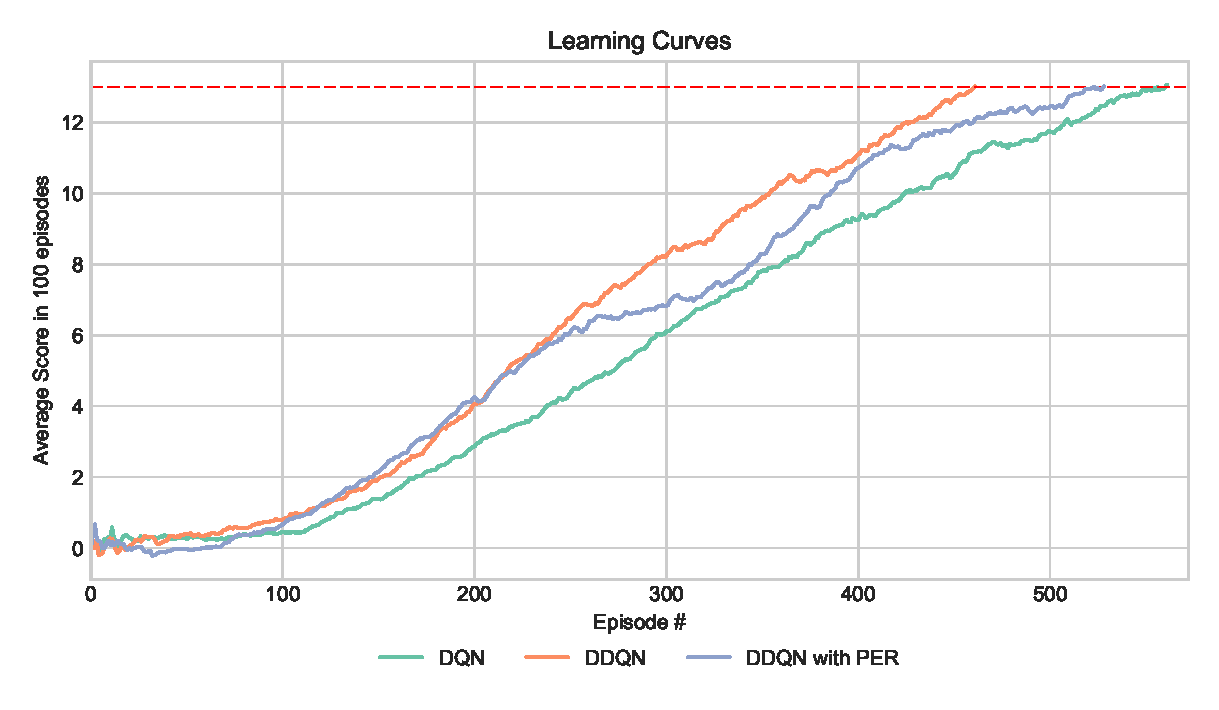
\includegraphics[width=0.65\textwidth]{../notebooks/figures/2018-08-23-final-comparition-2.eps}
\caption{Moving Average of $100$ episodes of the score}
\label{fig:final_comp}
\end{figure}

% The submission has concrete future ideas for improving the agent's performance.
Finally, as some possibles extensions, the parameters of the models could be better tuned and another models could be added to the analysis, as the Dueling network, presented by \cite{Wang:2015wz}, or the Rainbow, presented by \cite{Hessel:2017tw}, that  combines different improvements in Deep Reinforcement Learning, including the models presented in this project.



% ----------------end of document body---------------------

%---------------- start of references------------------

\bibliographystyle{plain}
% or try abbrvnat or unsrtnat
\bibliography{biblio.bib}

%---------------- end of references------------------


\end{document}
